\documentclass[11pt]{article}
\usepackage{geometry}                % See geometry.pdf to learn the layout options. There are lots.
\geometry{letterpaper}                   % ... or a4paper or a5paper or ... 
%\geometry{landscape}                % Activate for for rotated page geometry
%\usepackage[parfill]{parskip}    % Activate to begin paragraphs with an empty line rather than an indent
\usepackage{graphicx}
\usepackage{amssymb}
\usepackage{slashed}
\usepackage{epstopdf}
\usepackage{amsmath}
\DeclareGraphicsRule{.tif}{png}{.png}{`convert #1 `dirname #1`/`basename #1 .tif`.png}

\setlength{\parindent}{0pt}

\def\sp{\slashed{p}}
\def\sk{\slashed{k}}
\def\cn{\chi^0}
\def\cp{\chi^+}
\def\cm{\chi^-}
\def\gm{\gamma^{\mu}}
\def\gn{\gamma^{\nu}}
\def\gp{\gamma^{\rho}}
\def\km{k_{\mu}}
\def\kn{k_{\nu}}
\def\kp{k_{\rho}}
\renewcommand{\d}{\ensuremath{\operatorname{d}\!}}
\def\kmpm{k^{\mu}p_{\mu}}
\def\he{\frac{\epsilon}{2}}


\title{Relic density calculator documentation}


\begin{document}
\maketitle


\begin{figure}
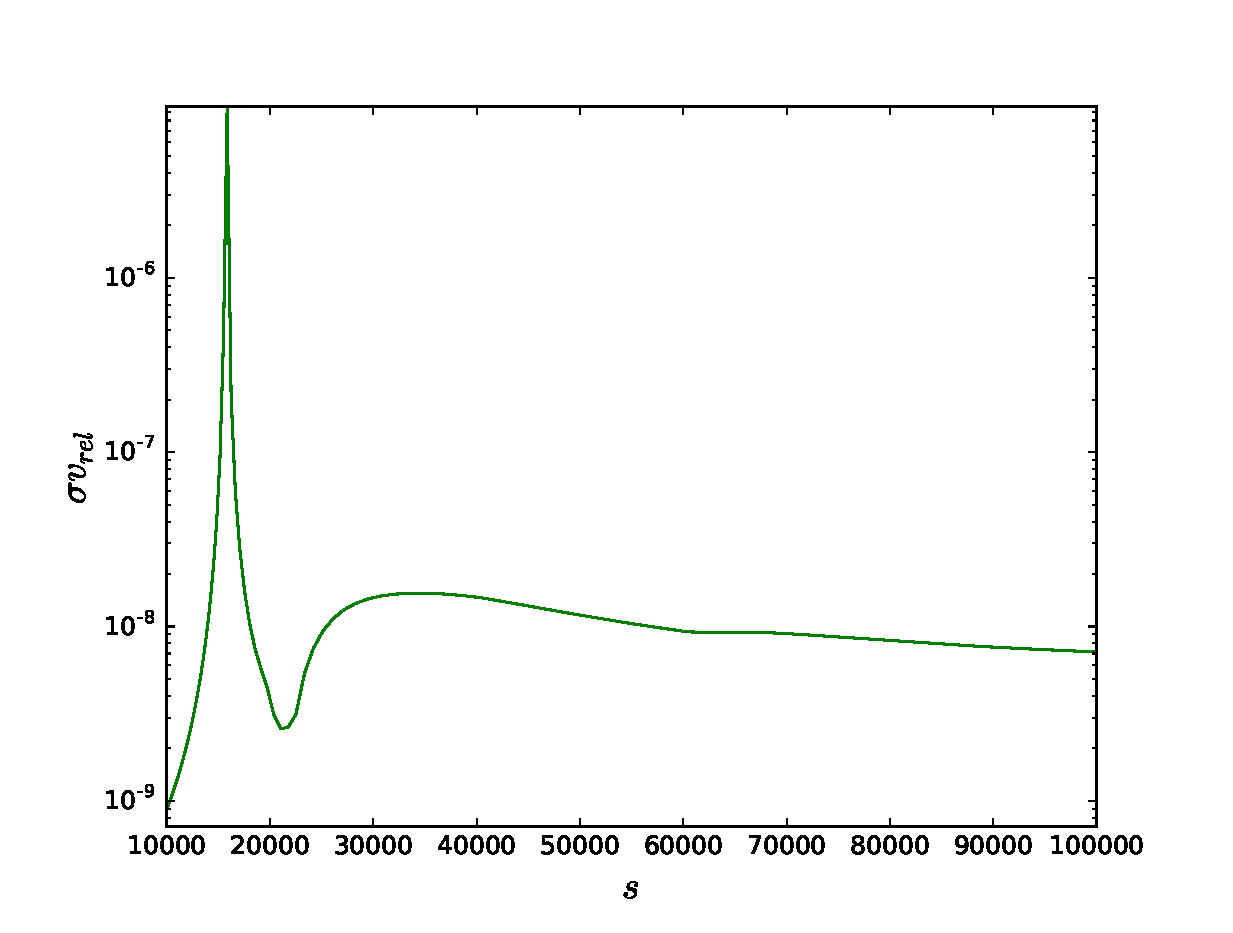
\includegraphics[width=0.5\textwidth]{resonance.eps}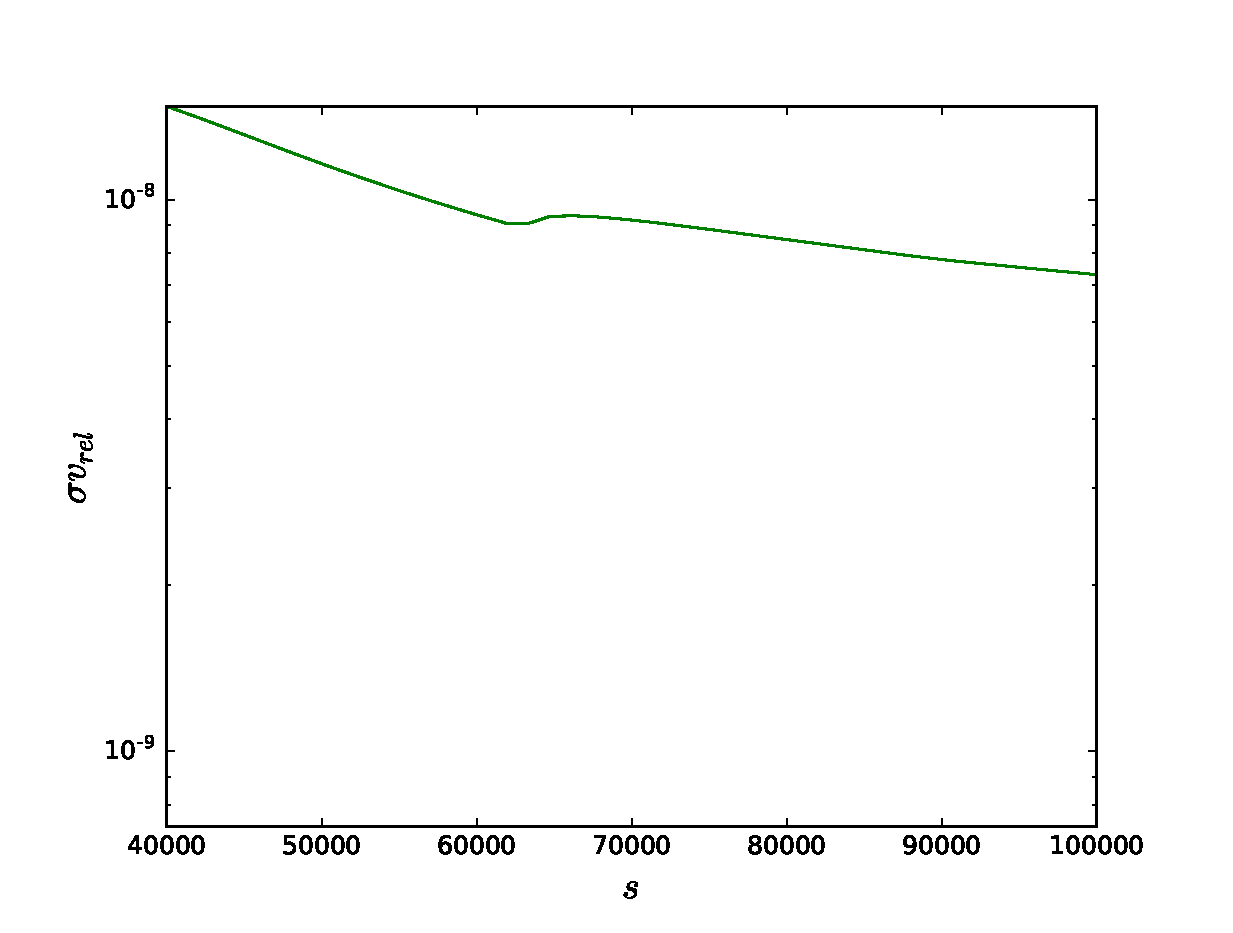
\includegraphics[width=0.5\textwidth]{no_resonance.eps}\label{fig:Higgs_res}
\caption{$\sigma v$, (\ref{eqn:sv}), as a function of $s$ for $m_s=50$ GeV (left) and $m_s=100$ GeV (right), where on the left we see a resonance at $s=m_h^2/4$ as expected.  Note that the vertical scale is very different on these two plots, and the far left point is $s=4m_s^2$ in each case.}
\end{figure}

In Figure \ref{fig:Higgs_res} we show the cross section for a scalar mass $m_s=50$ given by
\begin{align}
\sigma v_{rel}=\frac{2\lambda_{hs}^2v_0^2}{\sqrt{s}} |D_h(s)|^2\Gamma_h(\sqrt{s}) \label{eqn:sv}
\end{align}





\end{document}  